\documentclass[9pt]{article}
 
\usepackage{times}
\usepackage{transparency}
\usepackage[german]{babel}
\usepackage[T1]{fontenc}
\usepackage[latin1]{inputenc}
\usepackage{subfigure}

\screensize{8.5truein}{11truein}
\begin{document}


\title{On the Validation of Radio Propagation Models}

\setbackground{background.png}
\subtitle{Analytical validation of Network Simulator used\\Propagation and Bit Error Rates Models}

\name{Hagen Paul Pfeifer}
\footerline{Radio Propagation Models}
\email{hagen.pfeifer@protocollabs.de}
\company{ProtocolLabs\\http://www.protocollabs.com\\Munich, Germany}
\date{\today}
\maketitle

%%%%%%%%%%%%%%%%%%%%%%%%%%%%%%
\begin{slide}
\slidetitle{Disclaimer}{Disclaimer}
\bi
	\item The initial purpose of this work was to verify and
	      check the implementation of the \textit{Nakagami Fading Model}
		  in ns-3. In the half of the work I realized that the generated
		  material is a good starting point for path loss in general.
		  Especially to develop intuition how path loss influence the Wireless
		  simulation at the whole. How model knobs influences the
		  characteristic of the channel, etc.

	\item The complete work is public available and can be used for further
	      investigation:\newline
	      \verb+git clone http://git.jauu.net/wireless-propagation.git+

	\item Suggestion, enhancement or critic is highly welcome!
\ei
\end{slide}


%%%%%%%%%%%%%%%%%%%%%%%%%%%%%%
\begin{slide}
\slidetitle{Introduction}{Introduction}
\begin{picture}(0,0)
\put(100,-520){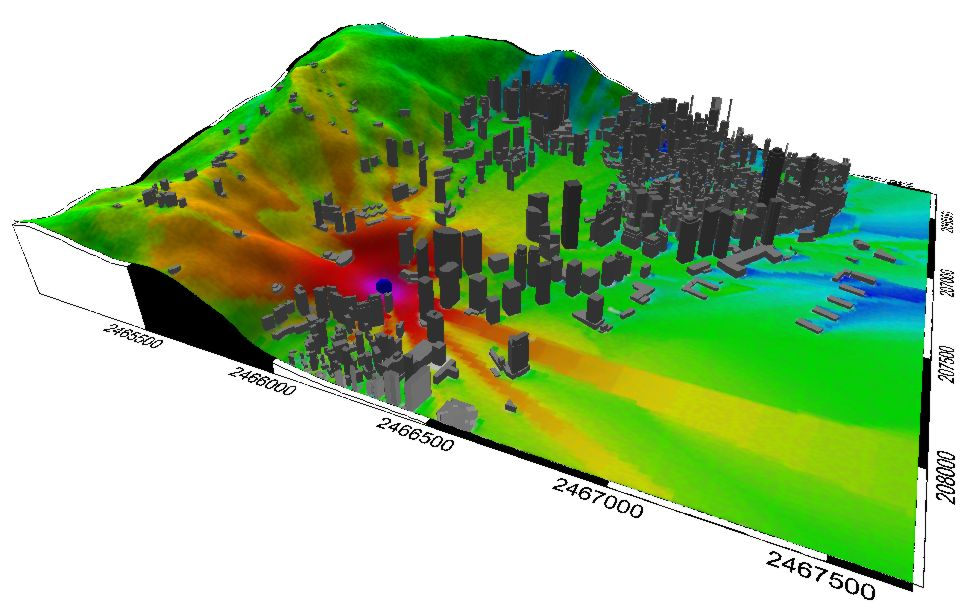
\includegraphics[scale=0.5]{images/hong-kong.jpg}}
\end{picture}
\bi
	\item A Wireless channel is unsteady and lossy
	\item Wireless network simulators requires a model of this characteristic
	\item Most relevant parameters for wave propagation:
	\be
		\item Attenuation
		\item Slow Fading (shadowing)
		\item Fast Fading (multipath scattering)
	\ee
	\item For the Symbol/Bit Error Rate (BER) the coding scheme is also of interest
\ei
\end{slide}

%%%%%%%%%%%%%%%%%%%%%%%%%%%%%%
\begin{slide}
\slidetitle{Fresnel Zone}{Fresnel Zone}
		\begin{picture}(0,0)
		\put(100,-450){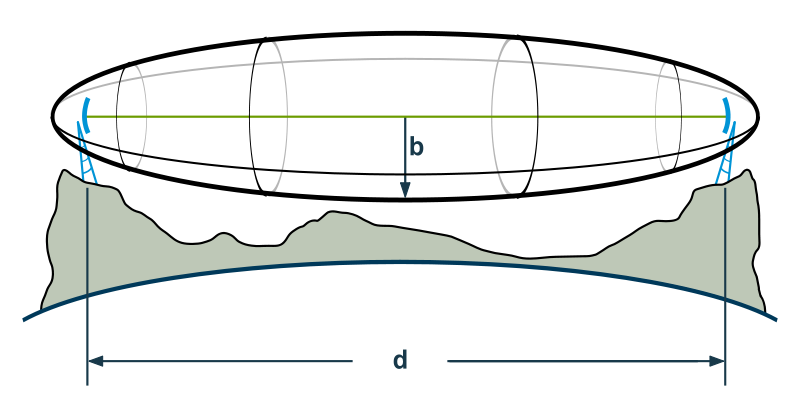
\includegraphics[scale=0.4]{images/fresnel.png}}
		\end{picture}
\bi
	\item The 1st Fresnel (pronounced Fray-nell) zone is a spheroid
	      with its center along both shortest distance between antennas.
	\item If there are no obstacles in the space forming 60\%
	      of this distance, propagation characteristics are said to be
		  the same as in free space
	\item Ensure line of sight between the transceivers
	\item If a Fresnel zone is not established, multipath interference will occur
	\item The Fresnelzone depends on the frequency: $>F \rightarrow{} <b$
	\item \begin{math} F_n = \sqrt{\frac{n \lambda d_1 d_2}{d_1 + d_2}} \end{math},
	      \begin{math} \lambda = \frac{v}{f}\end{math}
\ei
\end{slide}

%%%%%%%%%%%%%%%%%%%%%%%%%%%%%%
\begin{slide}
\slidetitle{Attenuation}{Attenuation}
\bi
	\item So how to calculate the attenuation of a channel?
	\item How to map slow- and fast fading conditions?
\ei
\end{slide}

%%%%%%%%%%%%%%%%%%%%%%%%%%%%%%
\begin{slide}
\slidetitle{Friis}{Friis}
\bi
	\item Friis is a transmission equation gives the power received by one antenna
	      under idealized conditions.
	\item Formula:\\\vspace{1cm}
	\begin{large}
	\begin{math}
	\frac{P_r}{P_t} = G_t G_r (\frac{\lambda}{4 \pi R} )^2
	\end{math}\\\vspace{1cm}
	\end{large}
	\begin{small}
	$P_r$ Receiving power (dBm)\\
	$P_t$ Transmitter power (dBm)\\
	$G_t$ Antenna Gain Transmitter (dBi/dBd)\\
	$G_r$ Antenna Gain Receiver (dBi/dBd)\\
	$\lambda$ Wavelength (meter, \dots)\\
	$R$ Distance between the nodes (meter, \dots)\\
	\end{small}
	\item But: ideal conditions are never achieved\footnote{one exception
	      is satellite communications when there is negligible atmospheric absorption}
\ei
\end{slide}

%%%%%%%%%%%%%%%%%%%%%%%%%%%%%%
\begin{slide}
		\begin{picture}(0,0)
		\put(100,-400){\includegraphics[scale=0.7]{images/friis.pdf}}
		\end{picture}
\slidetitle{Friis}{Friis}
\end{slide}

%%%%%%%%%%%%%%%%%%%%%%%%%%%%%%
\begin{slide}
\slidetitle{Friis Wavelength Influences}{Friis Wavelength Influences}
			\begin{figure}[ht]
			\centering
			\subfigure[\tiny{Frequency: 900 Mhz (GSM)}]{\includegraphics[scale=0.45]{images/friis900.pdf}}
			\subfigure[\tiny{Frequency: 5.0 GHz (802.11)}]{\includegraphics[scale=0.45]{images/friis5000.pdf}}
			\end{figure}
\bi
	\item The higher the frequency, the higher the loss.
\ei
\end{slide}

%%%%%%%%%%%%%%%%%%%%%%%%%%%%%%
\begin{slide}
\begin{picture}(0,0)
\put(100,-400){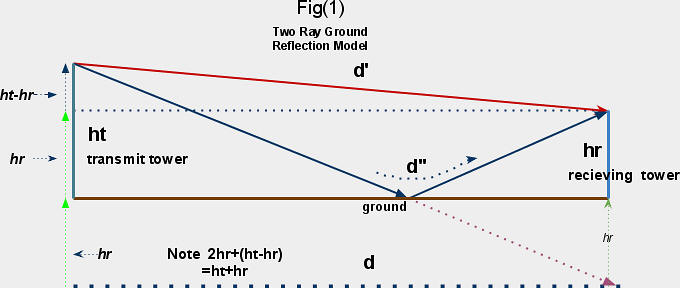
\includegraphics[scale=0.7]{images/two-ray-ground.png}}
\end{picture}
\slidetitle{Two Ray Ground}{Two Ray Ground}
\bi
	\item Friis at long distance tends to accurate prediction
	\item The single line-of-sight path is seldom the only means of propagation
	\item The two-ray ground reflection model considers both
	      the direct path and a ground reflection path
	\item \begin{math} P_r(d) = \frac{P_t G_t G_r h_t^2 h_r^2}{d^4 L} \end{math}
	\bi
		\item $L$: 1
	\ei
	\item Increased power loss compared to Free Space Model
	\item No good results for small distance $\rightarrow$ use Free Space Model
	      for near distances
\ei
\end{slide}

%%%%%%%%%%%%%%%%%%%%%%%%%%%%%%
\begin{slide}
		\begin{picture}(0,0)
		\put(100,-400){\includegraphics[scale=0.7]{images/tworaygroundvanilla.pdf}}
		\end{picture}
\slidetitle{Two Ray Ground (vanilla)}{Two Ray Ground (vanilla)}
\end{slide}

%%%%%%%%%%%%%%%%%%%%%%%%%%%%%%
\begin{slide}
		\begin{picture}(0,0)
		\put(100,-400){\includegraphics[scale=0.7]{images/tworayground.pdf}}
		\end{picture}
\slidetitle{Two Ray Ground}{Two Ray Ground}
\end{slide}

%%%%%%%%%%%%%%%%%%%%%%%%%%%%%%
\begin{slide}
		\begin{picture}(0,0)
		\put(100,-400){\includegraphics[scale=0.7]{images/logdistance.pdf}}
		\end{picture}
\slidetitle{Log Distance Model}{Log Distance Model}
\end{slide}

%%%%%%%%%%%%%%%%%%%%%%%%%%%%%%
\begin{slide}
\begin{picture}(0,0)
\put(100,-400){\includegraphics[scale=0.7]{images/threelogdistance.pdf}}
\end{picture}
\slidetitle{Three Log Distance Model}{Three Log Distance Model}
\end{slide}

%%%%%%%%%%%%%%%%%%%%%%%%%%%%%%
\begin{slide}
\slidetitle{Fading}{Fading}
		\begin{picture}(0,0)
		\put(350,-190){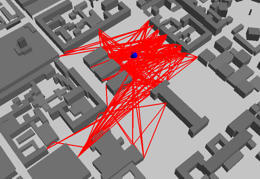
\includegraphics[scale=1.]{images/urban.png}}
		\end{picture}
\bi
	\item Fading is deviation of the attenuation
	\item Reasons:
	\bi
		\item Shadowing from obstacles
		\item Multipath propagation
	\ei
	\item Slow Fading
	\bi
		\item Roughly constant amplitude and phase change over time
		\item Hills, buildings, \dots
		\item Often modeled using a log-normal distribution
	\ei
	\item Fast fading
	\bi
		\item Amplitude and phase change varies considerably
		\item Multiple reflections
	\ei
	\item Modeled as a random process
\ei
\end{slide}


%%%%%%%%%%%%%%%%%%%%%%%%%%%%%%
\begin{slide}
		\begin{picture}(0,0)
		\put(100,-400){\includegraphics[scale=0.7]{images/shadowing.pdf}}
		\end{picture}
\slidetitle{Shadowing Model}{Shadowing Model}
\end{slide}

%%%%%%%%%%%%%%%%%%%%%%%%%%%%%%
\begin{slide}
		\begin{picture}(0,0)
		\put(100,-400){\includegraphics[scale=0.7]{images/nakagami.pdf}}
		\end{picture}
\slidetitle{Nakagami Model}{Nakagami Model}
\end{slide}

%%%%%%%%%%%%%%%%%%%%%%%%%%%%%%
\begin{slide}
		\begin{picture}(0,0)
		\put(100,-400){\includegraphics[scale=0.7]{images/nakagami_distribution.pdf}}
		\end{picture}
\slidetitle{Nakagami Model Distribution}{Nakagami Model Distribution}
\end{slide}

%%%%%%%%%%%%%%%%%%%%%%%%%%%%%%
\begin{slide}
		\begin{picture}(0,0)
		\put(100,-400){\includegraphics[scale=0.7]{images/nakagami_m0_variances.pdf}}
		\end{picture}
\slidetitle{Nakagami Model m0 Effect}{Nakagami Model m0 Effect}
\end{slide}

%%%%%%%%%%%%%%%%%%%%%%%%%%%%%%
\begin{slide}
		\begin{picture}(0,0)
		\put(100,-400){\includegraphics[scale=0.7]{images/nakagami_m0_variance_distribution.pdf}}
		\end{picture}
\slidetitle{Nakagami Model m0 Effect}{Nakagami Model m0 Effect}
\end{slide}

%%%%%%%%%%%%%%%%%%%%%%%%%%%%%%
\begin{slide}
\slidetitle{RX Power to SNR}{RX Power to SNR (1/2)}
\bi
	\item Signal-to-Noise Ratio (SNR or S/N)
	\item Ratio of a signal power to the noise power corrupting the signal
	\item $SNR = \frac{P_{signal}}{P_{noise}}$
	\item Noise:
	\bi
		\item Boltzmann constant * Bandwidth * Receiver Noise * Implementation Loss
		\item Boltzmann constant ($k_B$): $3.91^{-21}$ (B * Temp in Kelvin)
		\item Bandwidth: $20^6$ Hz
		\item Receiver Noise: 15.8 W (~12 dB)
		\item Implementation Loss: 1.58 W (2 dB)
	\ei
\ei
\end{slide}

%%%%%%%%%%%%%%%%%%%%%%%%%%%%%%
\begin{slide}
\slidetitle{RX Power to SNR}{RX Power to SNR (2/2)}
\bi
	\item Noise: $1.99^{-12}$ Watt = $-87 dBm$
	\item Example:
	\bi
		\item Signal: -60 dBm
		\item Noise: -87 dBm
		\item SNR: -27 dB
	\ei
\ei
\end{slide}



%%%%%%%%%%%%%%%%%%%%%%%%%%%%%%
\begin{slide}
\slidetitle{Symbol/Bit Error Rate}{Symbol/Bit Error Rate (1/2)}
\bi
	\item Symbol Error Rate
	\item Common digital modulation schemes:
	\bi
		\item Binary phase-shift keying (BPSK, 2 Symbols)
		\item Quadrature phase-shift keying (QPSK, 4 Symbols)
		\item 8 Phase-shift keying (8PSK, 8 Symbols)
		\item $n$-Quadrature amplitude modulation (QAM, 16, 32, 64 Symbols)
		\item \dots
	\ei
\ei
\end{slide}


%%%%%%%%%%%%%%%%%%%%%%%%%%%%%%
\begin{slide}
\slidetitle{Symbol/Bit Error Rate}{Symbol/Bit Error Rate (2/2)}
\begin{picture}(0,0)
\put(-260,-480){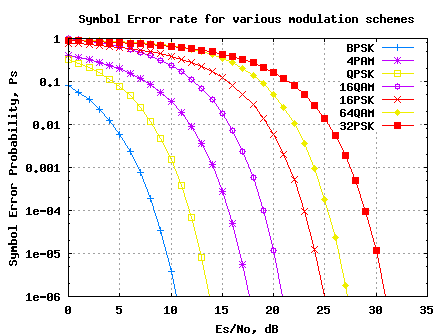
\includegraphics[scale=.7]{images/srr.png}}
\end{picture}
\bi
	\item Symbol Error Rate vs. Es/No
	\item \begin{math} P_{S,MQAM} = 2 ( 1 - \frac{1}{\sqrt{M}} )  erfc( \sqrt{ \frac{3}{2(M-1)} \frac{E_s} {E_0} }) - ( 1 -
	\frac{2}{\sqrt{M}} + \frac{1}{M}) erfc^2 (\sqrt{\frac{3}{2-(M-1)} \frac{E_s}{E_0}}) \end{math}
	\item Inverse Error Function (also known as Gauss error function):
	\bi
	\item \begin{math}erfc(x) = \frac{2}{\sqrt{\pi}} \int^\infty_x e^{-t^2}dt\end{math}
	\ei
	\item Symbol Error Rate $\rightarrow$ Bit Error Rate: $\frac{P_{S,MQAM}}{Bits per Symbol}$
\ei
\end{slide}

%%%%%%%%%%%%%%%%%%%%%%%%%%%%%%
\begin{slide}
\slidetitle{The End}{The End}
\bi
	\item Questions?
\ei
\end{slide}

%%%%%%%%%%%%%%%%%%%%%%%%%%%%%%
\begin{slide}
\slidetitle{SINR and IPW2200}{SINR and IPW2200}
\bi
	\item Signal-To-Noise Ratio (aka SNR and S/R)
	\item snr(dB) = signal level(dBm) - average noise level(dBm)
	\item Ratio of a signal power to the noise power corrupting the signal
	\item To receive a useful information the signal must clearly be higher then the noise
	\item Sidenote IPW2200 driver and \verb+/proc/net/wireless+
	\bi
		\item \verb+iwconfig eth1+ $\rightarrow$ Link Quality=69/100  Signal level=-55 dBm  Noise level=-82 dBm
		\item Noise: initial set to -85 dBm
		\item Every new packet updates the noise level (and average it with the previous one)
		\item \verb+priv->exp_avg_noise+
		\item RSSI: received signal strength indication
		\item RSSI: a measurement of the power present in a received radio signal
		\item 0 to 255
		\item RSSI is acquired during the preamble stage of receiving an 802.11 frame
		\item RSSI is stored on the RX descriptor (stats.rssi) and is measured by baseband and PHY for each individual packet
		\item see \verb+drivers/net/wireless/ipw2x00/ipw2200.c:ipw_rx()+
	\ei
\ei
\end{slide}

%%%%%%%%%%%%%%%%%%%%%%%%%%%%%%
\begin{slide}
\slidetitle{Some Background on Antennas}{Some Background on Antennas}
\begin{picture}(0,0)
\put(50,-200){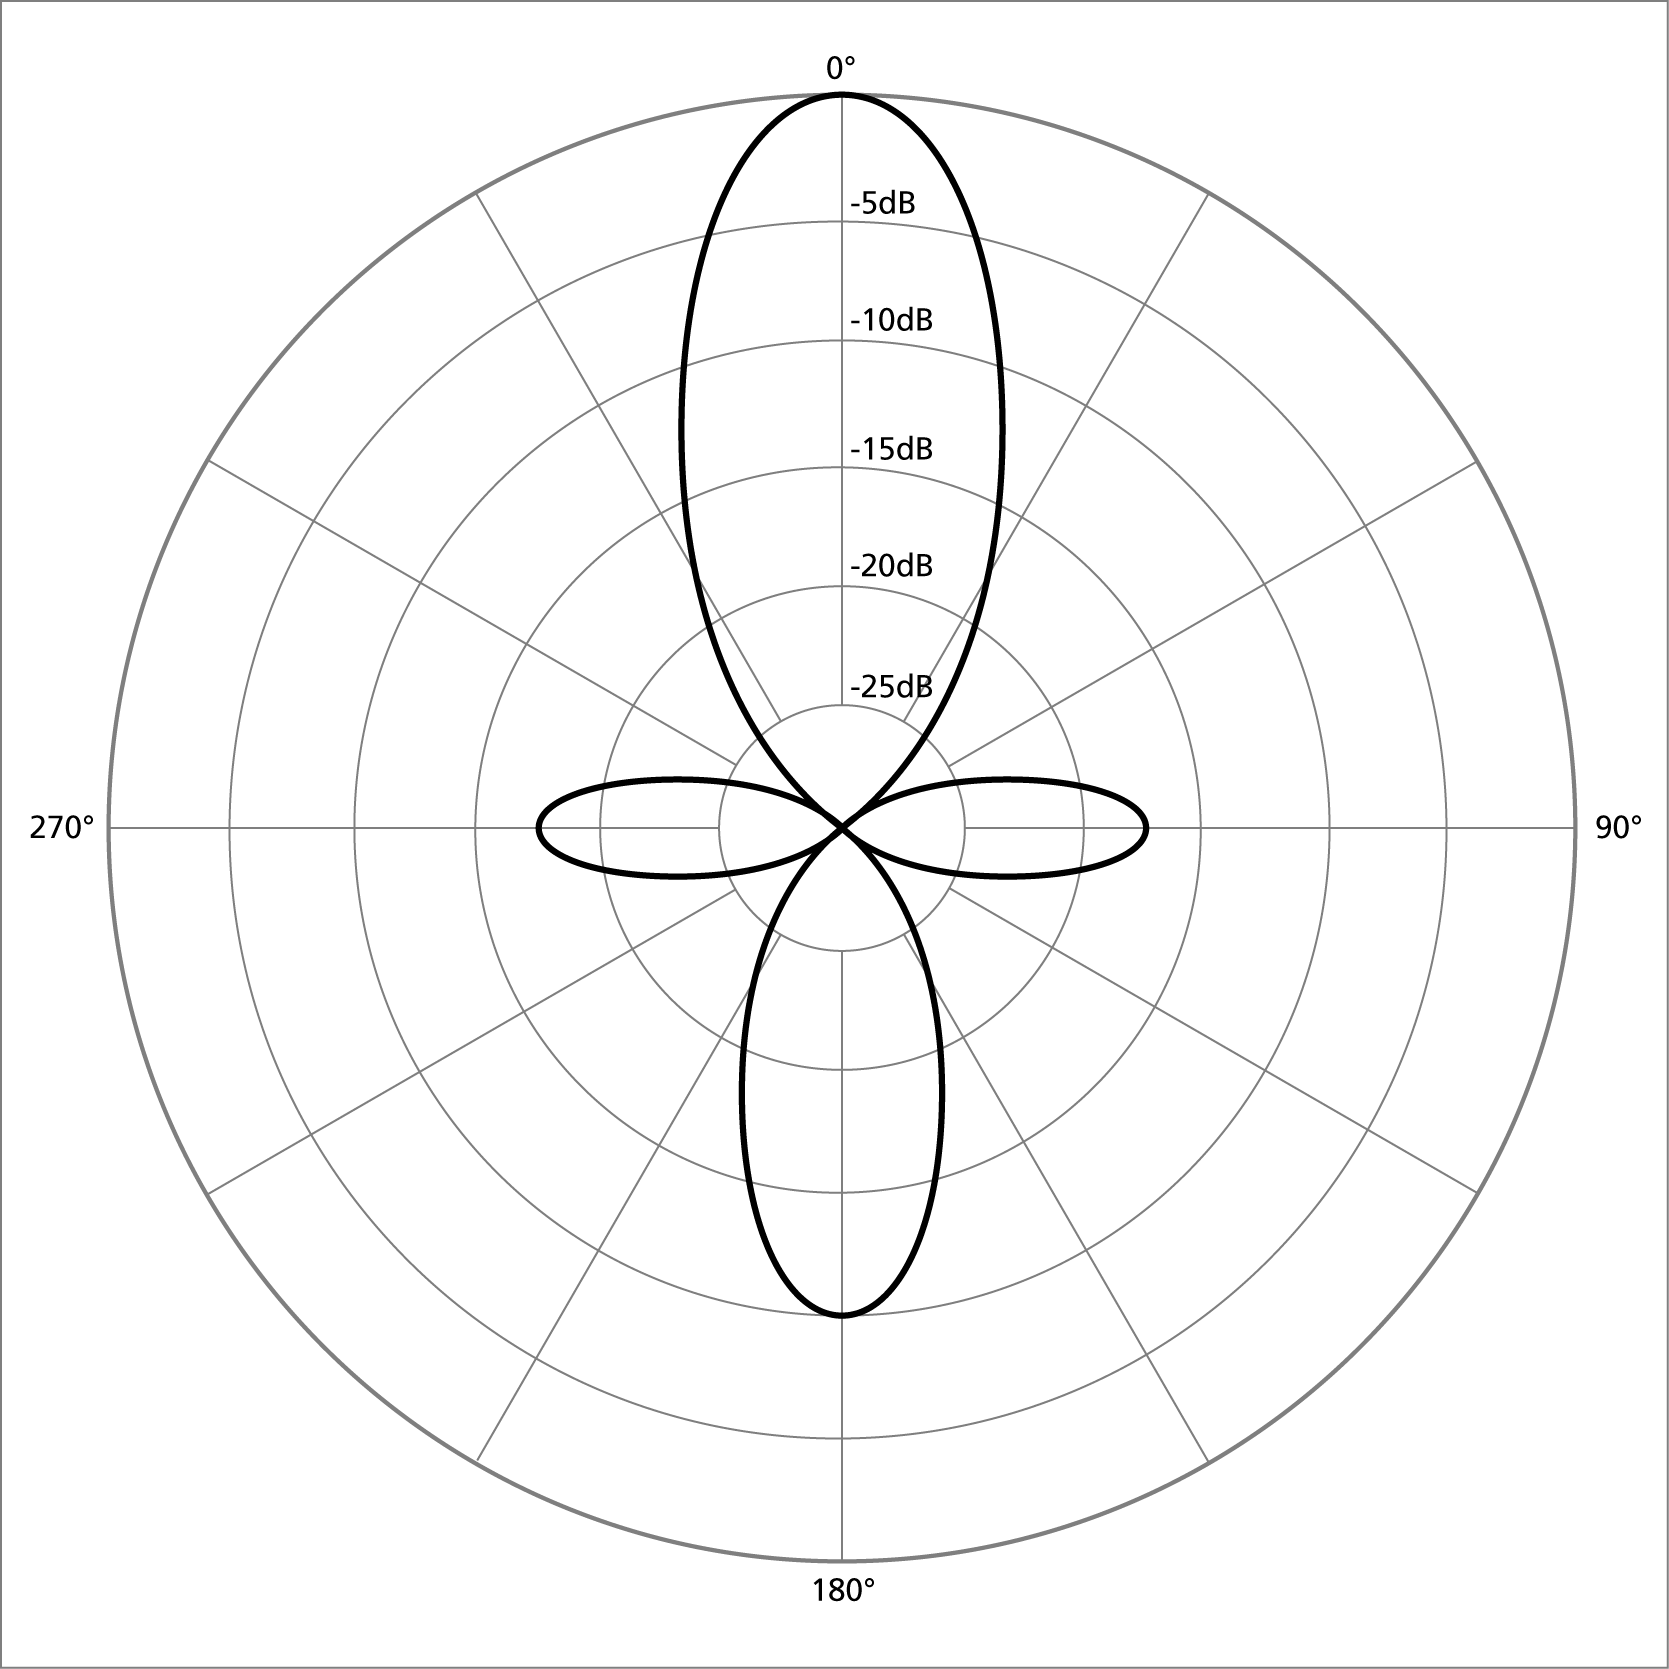
\includegraphics[scale=0.25]{images/polar_pattern_directional.png}}
\end{picture}
\begin{picture}(0,0)
\put(50,-450){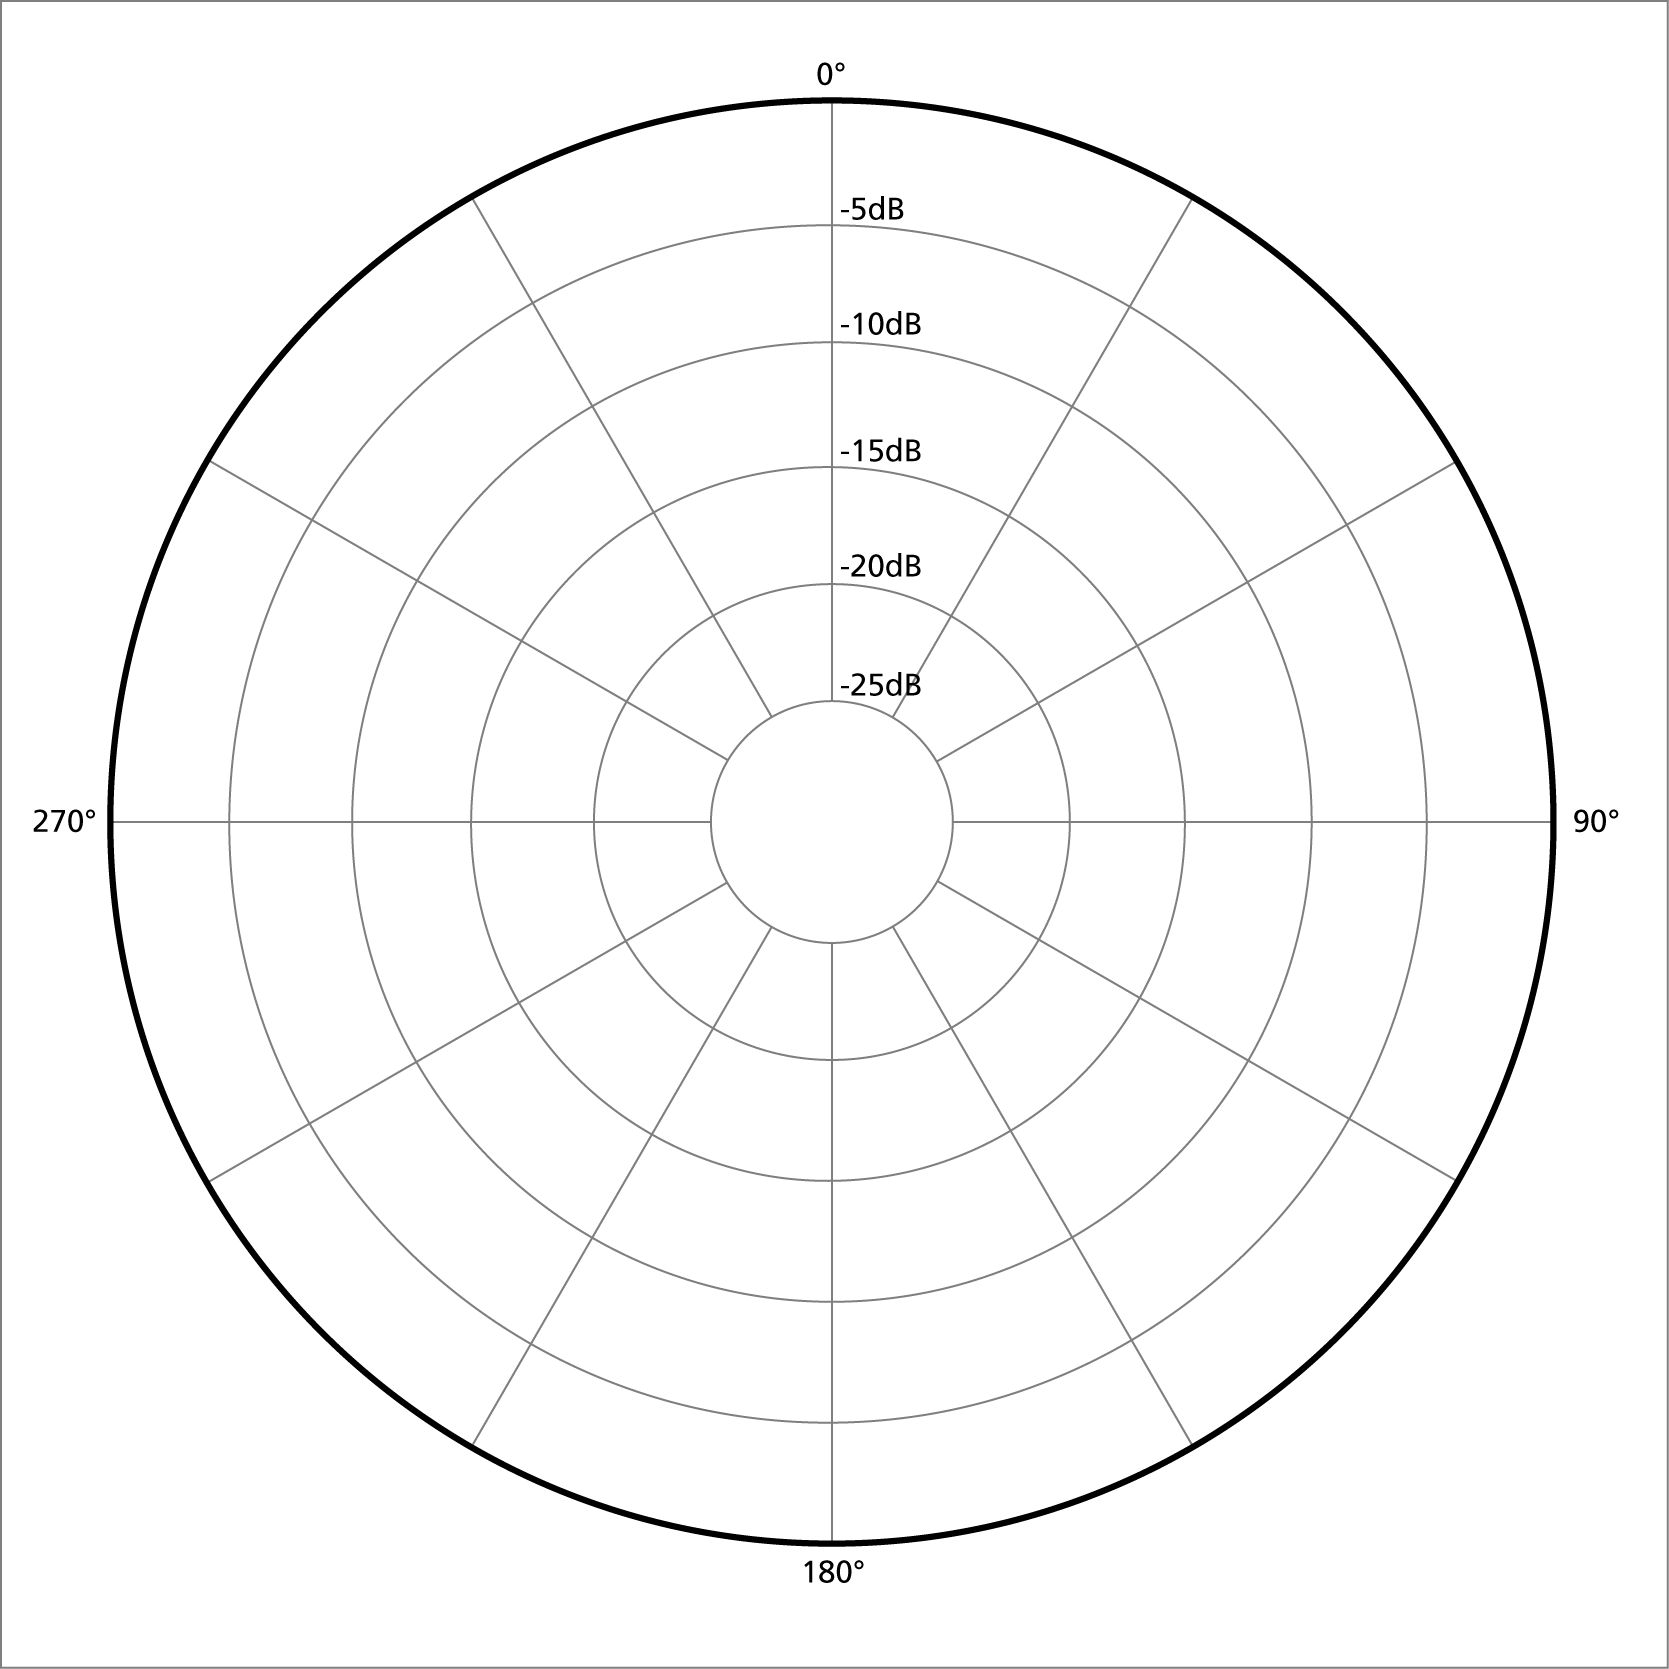
\includegraphics[scale=0.25]{images/polar_pattern_omnidirectional.png}}
\end{picture}
\bi
	\item Basic types
	\bi
		\item Omnidirectional
		\item Semi-directional
		\item Directional
	\ei
	\item Omnidirectional
	\bi
		\item Omnidirectional antennas radiate energy equally in  all directions around the antenna's vertical axis
		\item Most common for WLAN: dipole antenna
	\ei
	\item Semi-Directional
	\bi
		\item Patch
		\item Panel
		\item Yagi
		\item Common examples: TV antennas or Cellular repeaters antennas
	\ei
	\item Highly Directional
	\bi
		\item Parabolic dish
		\item Grid antenna
	\ei
\ei
\end{slide}

%%%%%%%%%%%%%%%%%%%%%%%%%%%%%%
\begin{slide}
\slidetitle{Common dbM/Watt Values}{Common dbM/Watt Values\footnote{Source: WP}}
\bi
	\item 80 dBm	100 kW	Typical transmission power of FM radio station with 50 km range
	\item 60 dBm	1 kW = 1000 W	Typical combined radiated RF power of microwave oven elements
	\item 33 dBm	2 W		Maximum output from a UMTS/3G mobile phone (Power class 1 mobiles)
	\item 30 dBm	1 W = 1000 mW	Typical RF leakage from a microwave oven
	\item 20 dBm	100 mW	Bluetooth Class 1 radio, 100 m range
	\item 15 dBm    32 mW	Typical WiFi transmission power in laptops
	\item  4 dBm     2.5 mW	Bluetooth Class 2 radio, 10 m range
	\item  0 dBm     1.0 mW = 1000 $mu$W	Bluetooth standard (Class 3) radio, 1 m range
	\item -10 dBm   100 $mu$W	Typical maximum received signal power (-10 to -30 dBm) of wireless network
	\item -70 dBm   100 pW	Typical range (-60 to -80 dBm) of wireless (802.11x) received signal power over a network
	\item -127.5 dBm	0.178 fW = 178 aW	Typical received signal power from a GPS satellite
	\item -174 dBm	0.004 aW = 4 zW		Thermal noise floor for 1 Hz bandwidth at room temperature (20 C)
\ei
\end{slide}

\end{document}

% vim600: fdm=marker tw=130 sw=4 ts=4 sts=4 ff=unix noet:
